\chapter{Introduction}
\label{cha:intro}

\begin{figure}[htb!]
	\centering
	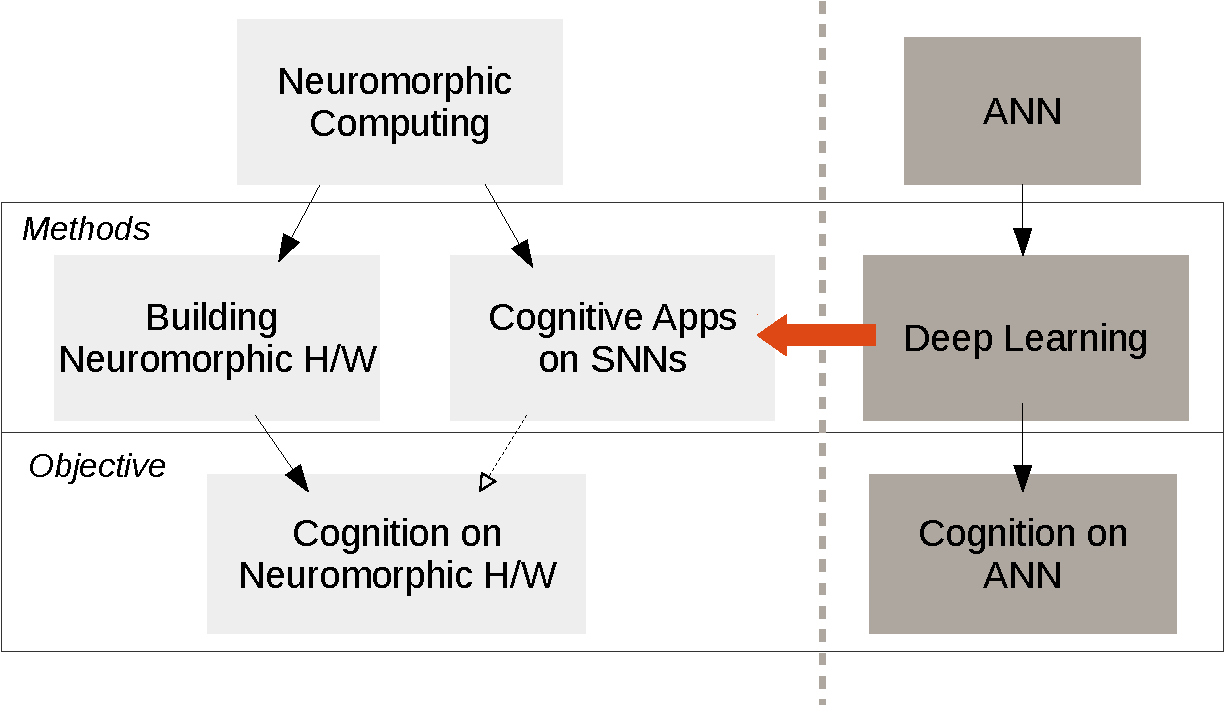
\includegraphics[width=0.8\textwidth]{pics_intro/intro.pdf}
	\caption{The story line of the thesis.}
	\label{fig:intro}
\end{figure}

%Problem, motivation and significance
%TODO neuromorphic computing
%Initial aim

%development with hardware, about SpiNNaker, DVS

%TODO SNN, focus on neural science simulation, mention plasticity

%TODO ANN
%deep learning fruitful results

%TODO merge objectives
%how I find the problem

%Why it motivates me (why it would be useful and important to have a solution)



\section{Statement of The Problem}
\label{sec:problem}
Neuromorphic computing has lead towards the development of biologically-inspired computer architectures which may alternate conventional Von Neumann and rival the Human brain in terms of energy efficiency and cognitive capabilities.
Although there are a number of neuromorphic platforms available for large-scale SNN simulations, how to operate these brain-like machines to be competent in cognitive applications still remains unsolved.
While Deep Learning within the research of ANNs has dominated the state-of-the-art solutions on AI applications and machine learning.
SNN has not achieved the cognitive capability and learning ability of its non-spiking competitor, ANN.
To reduce the gap of cognitive performance is the main objective of this research.


\section{Hypotheses and Aims}
\label{sec:aim}
The main objective is to improve the cognitive capability and equip the equivalent learning ability of SNNs as ANNs' for AI applications.
In addition, to run such a biologically-plausible model on complete hardware platform validates the feasibility of real-time Neuromorphic Computing over cognitive tasks.
Moreover, it is necessary to provide the community a uniform dataset and an evaluation methodology to compare the performance of SNN models and hardware platforms.

\begin{itemize}
	\item 
	An object recognition system can operate in real-time on a complete neuromorphic platform in an absolute spike-based fashion.
	The hypothesis pave the way for further study with solid proof of the capability of real-time cognitive application built on neuromorphic platform.

	Aim: to build a real-time neuromorphic object recognition prototype running on hardware SNN simulator and receiving visual input from a DVS sensor.

	\item 
	SNNs can deliver equivalent cognitive capability as conventional ANNs for object recognition applications.

	Aim: to generalise a training method on conventional ANNs whose trained connections can be applied to corresponding SNNs with close recognition performance.

	\item 
	SNNs can be trained with biologically-realistic synaptic plasticity and demonstrate competent learning capability as ANNs, even as state-of-the-art deep architectures.

	Aim: to formalise a local learning algorithm based on synaptic plasticity for training deep SNNs.

	\item 
	A new set of spike-based vision datasets can provide resources to support fair competition between researchers since new concerns on energy efficiency and recognition latency emerge in Neuromorphic Vision.

	Aim: to provide a unified spiking version of common-used dataset and complementary evaluation methodology to assess the performance of SNN algorithms.
\end{itemize}


\section{Contributions}
The primary achievements of the thesis are the learning methods both off-line and on-line for SNNs, which close the gap of cognitive capability between SNNs and ANNs.
The other achievements contributes to the concerns of the feasibility of neuromorphic hardware platforms and the performance evaluation.
\begin{itemize}
	\item 
	An implementation of a real-time hand postures recognition system on a neuromorphic hardware platform.
	It demonstrated the prototype of a complete neuromorphic system which may form the default configuration of a real-time, energy-efficient and low-latency recognition system.
	
	This work comprises Chapter 3 and was published and presented to the International Conference on Artificial Neural Networks 2015.
	
	\item 
	A novel activation function, Noisy Softplus, to replace ReLU for training SNNs off-line.
	Network training with Noisy Softplus is a generalised method and the activation function can be applied in any architecture of a neural network theoretically.
	It was tested on a convolutional network and showed a close recognition capability comparing to the conventional ANN. 

	This work comprises Chapter 4 and was published and presented to International Conference on Neural Information Processing 2016.

	\item 
	A novel unsupervised learning algorithm purely working on event-based local STDP.
	The algorithm was applied to train an Autoencoder (AE) and a Restricted Boltzmann Machine (RBM).
	The learning ability matched the non-spiking ANNs and verified the feasibility of unsupervised training on deep SNNs. 
	
	This work comprises Chapter 5.
	A paper on these findings is in preparation to submit to International Joint Conference on Neural Network 2017.
	
	\item 
	A dataset and the corresponding evaluation methodology for comparisons of Neuromorphic Vision.
	This dataset also made the comparison of SNNs with conventional recognition methods possible by using converted spike representations of the same vision databases.
	As far as we know, this was the first attempt at benchmarking neuromorphic vision recognition by providing public a spike-based dataset and evaluation metrics.
	
	The dataset was generated by the help of Garibaldi~Pineda-Garc\'ia and Teresa~Serrano-Gotarredona, and the second case study was analysed by Evangelos~Stromatias.
	This work comprises Chapter 6 and was accepted as a journal paper of Frontiers in Neuromorphic Engineering.
\end{itemize}

   
\section{Publications and Workshops}
\subsection{Publications}
\begin{itemize}
	\item 
	\textbf{Q. Liu}, and S. Furber, “Real-Time Recognition of Dynamic Hand Postures on a Neuromorphic System”, International Conference on Artificial Neural Networks (ICANN 2015).
	The paper mainly comprises the work of Chapter~3.
	
	\item 
	\textbf{Q. Liu}, and S. Furber, “Noisy Softplus: A Biology Inspired Activation Function”, International Conference on Neural Information Processing (ICONIP 2016). 
	The paper mainly comprises the work of Chapter~4.
	
	
	\item 
	\textbf{Q. Liu}, and S. Furber, “STDP Training on Rate-Based Spiking Autoencoders”, International Joint Conference on Neural Network (to submit to IJCNN 2017).
	The paper mainly comprises the work of Chapter~5.
	
	\item 
	\textbf{Q. Liu}, G. Garcis, E. Stromatias, T. Gotarredona, and S. Furber, “Benchmarking Spike-Based Visual Recognition: A Dataset and Evaluation,” Frontiers in Neuromorphic Engineering.
	The paper comprises the work of Chapter~6.
	

	\item 
	G. Garcis, P. Camilleri, \textbf{Q. Liu}, and S. Furber, “pyDVS: A real-time dynamic vision sensor emulator using off-the-shelf hardware”, The 2016 IEEE Symposium Series on Computational Intelligence (IEEE SSCI 2016).
	
	\item
	\textbf{Q. Liu}, C. Patterson, S. Furber, Z. Huang, Y. Hou and H. Zhang, “Modeling Populations of Spiking Neurons for Fine Timing Sound Localization”, International Joint Conference on Neural Networks (IJCNN 2013)
\end{itemize}	

\subsection{Workshops}
It is essential for the author to participate in the workshops organised by the close community, 1) to establish and contribute to collaborations on mutual interests; 2) to catch up with the cutting-edge research and collect inspiration; 3) to discuss the author's own findings with the key researchers in the field.
\begin{itemize}
	\item 
	\textit{Capo Caccia Cognitive Neuromorphic Engineering Workshop 2012}.
	
	Contributed to successfully connections of SpiNNaker to neuromorphic sensors\footnote{\url{https://capocaccia.ethz.ch/capo/wiki/2012/csnQian}}. 
	It formed the hardware platform for real-time SNN applications processing event-based sensor data.
	
	\item 
	\textit{Telluride Neuromorphic Cognition Engineering Workshop 2013}.
	
	Developed a real-time sound localisation system on the neuromorphic platform as a main contributor\footnote{\url{http://neuromorphs.net/nm/wiki/sound_localization}}.
	The work led to the publication of a journal paper\cite{lagorce2015breaking}.
	
	
	\item 
	\textit{Capo Caccia Cognitive Neuromorphic Engineering Workshop 2014}.
	
	Developed the real-time neural activity visualiser for the project of ``Integrated Neurorobotics for Real-World Cognitive Behaviour'' \footnote{\url{https://capocaccia.ethz.ch/capo//wiki/2014/integrneurobot14}}. 
	
	\item 
	\textit{Capo Caccia Cognitive Neuromorphic Engineering Workshop 2015}.
	
	Fully inspired by the projects of deep learning in the workshop\footnote{\url{https://capocaccia.ethz.ch/capo//wiki/2015/spikednn15}}, the author later proposed the translation methods and the unsupervised learning algorithm of spiking deep networks.
	And led the discussion of benchmarking neuromorphic vision in the workshop \footnote{\url{https://capocaccia.ethz.ch/capo//wiki/2015/visionbenchmark15}}. 	
\end{itemize}
\section{Thesis Structure}
The thesis comprises the following seven chapters:

\textbf{Chapter 1} introduces the origin and the motivation of the research, states the problem, defines the hypotheses and objectives, summarises the contributions and publications, and outlined the thesis. 

\textbf{Chapter 2} briefs the short history of Neuromorphic Computing which leads to the author's research, lists the common spiking neural models and learning approaches, introduces the neuromorphic hardware devices and reviews the state-of-the-art of spike-based object recognition applications. 

\textbf{Chapter 3} is the first contribution content of the thesis, which details the implementation of the dynamic hand posture recognition system on a neuromorphic hardware; and describes the performance of both the real-time simulation and the live recognition. 

\textbf{Chapter 4} demonstrates the novel biologically-inspired activation function, Noisy Softplus, which is well-matched to the response function of Leaky Integrate-and-Fir neurons; and validates the performance by testing on a convolutional network.

\textbf{Chapter 5} proposes the STDP-based learning algorithm for training AEs and RBMs; and shows equivalent recognition capability of SNNs comparing to ANNs.

\textbf{Chapter 6} puts forward the spike-based vision dataset and the evaluation methodology; and presents two case studies as tentative benchmarks running on SpiNNaker to assess the hardware-level performance against software simulators.

\textbf{Chapter 7} summarises the research, discusses the contributions to the field, points out the future direction and concludes the thesis.



